\documentclass[10pt]{beamer}

\usepackage[brazilian]{babel}
\usepackage[utf8]{inputenc}
\usepackage{graphicx}
\usepackage{mathtools}
\usepackage{amsthm}
\usepackage{thmtools,thm-restate}
\usepackage{amsfonts}
\usepackage{hyperref}
\usepackage[singlelinecheck=false]{caption}
\usepackage[backend=biber,url=true,doi=true,eprint=false,style=alphabetic]{biblatex}
\usepackage[justification=centering]{caption}
\usepackage{indentfirst}
\usepackage{enumitem}
\usepackage{algorithm}
\usepackage{algpseudocode}
\usepackage{listings}
% Timeline
\usepackage{xcolor}
\newcommand\ytl[2]{
\parbox[b]{8em}{\hfill{\color{cyan}\bfseries\sffamily #1}~$\cdots\cdots$~}\makebox[0pt][c]{$\bullet$}\vrule\quad \parbox[c]{7.5cm}{\vspace{2pt}\color{red!40!black!80}\raggedright\sffamily #2.\\[7pt]}\\[-3pt]}

% Fix beamer and enumitem conflicts.
\setitemize{label=\usebeamerfont*{itemize item}%
  \usebeamercolor[fg]{itemize item}
\usebeamertemplate{itemize item}}

% Remove line breaks.
\setbeamertemplate{bibliography entry title}{}
\setbeamertemplate{bibliography entry location}{}
\setbeamertemplate{bibliography entry note}{}

\uselanguage{Brazilian}
\languagepath{Brazilian}
\usetheme{Berlin}

\addbibresource{references.bib}

\newcommand\nmfootnote[1]{%
  \begingroup
  \renewcommand\thefootnote{}\footnote{#1}%
  \addtocounter{footnote}{-1}%
  \endgroup
}

\makeatletter
\def\subsection{\@startsection{subsection}{3}%
  \z@{.5\linespacing\@plus.7\linespacing}{.1\linespacing}%
  {\normalfont}}
\makeatother

\DeclareMathOperator*{\argmin}{arg\,min}
\DeclareMathOperator*{\argmax}{arg\,max}

\newcommand\defeq{\mathrel{\overset{\makebox[0pt]{\mbox{\normalfont\tiny\sffamily def}}}{=}}}

\floatname{algorithm}{Algoritmo}
\algrenewcommand\algorithmicrequire{\textbf{Input}}
\algrenewcommand\algorithmicensure{\textbf{Output}}

\captionsetup[table]{labelsep=space}

\theoremstyle{plain}

\newtheorem{proposition}{Proposição}
\newtheorem{exercise}{Exercício}

\newcommand{\set}[1]{\mathbf{#1}}
\newcommand{\pr}{\mathbb{P}}
\renewcommand{\implies}{\Rightarrow}

\newcommand{\bigo}{\mathcal{O}}
\newcommand{\p}{\pause}

\setlength{\parskip}{1em}

\lstset{frameround=fttt,
  language=[5.3]Lua,
  numbers=left,
  breaklines=true,
  keywordstyle=\bfseries,
  basicstyle=\ttfamily,
}

\newcommand\Fontsmall{\fontsize{12}{7.2}\selectfont}

\newcommand{\code}[1]{\lstinline[mathescape=true]{#1}}
\newcommand{\mcode}[1]{\lstinline[mathescape]!#1!}

\title{GNU Hurd}
\subtitle{MAC0422 --- Estudo de Caso}
\author{Renato Lui Geh\\ NUSP:\@ 8536030}

\begin{document}

\frame{\titlepage}

\begin{frame}
  \frametitle{Índice}
  \tableofcontents
\end{frame}

%--------------------------------------------------------------------------------------------------

\section{História}

\begin{frame}
  \frametitle{História do GNU/Hurd}

  \begin{table}
    \begin{minipage}[t]{\linewidth}
      \color{gray}
      \rule{\linewidth}{1pt}
      \ytl{1983}{Richard Stallman (RMS) cria o projeto GNU}
      \ytl{1986}{RMS decide usar o TRIX como kernel}
      \ytl{1988}{É decidido usar o Mach como kernel}
      \ytl{1991}{GNU Hurd é anunciado ao público}
      \ytl{1994}{Primeiro boot}
      \ytl{1994}{Emacs e gcc rodam pela primeira vez}
      \ytl{1995}{ext2fs, ftp}
      \ytl{1996}{NFS e GNU Hurd 0.1}
      \ytl{1997}{GNU Hurd 0.2}
      \bigskip
      \rule{\linewidth}{1pt}
    \end{minipage}
  \end{table}

\end{frame}

\begin{frame}
  \frametitle{História do GNU/Hurd}

  \begin{table}
    \begin{minipage}[t]{\linewidth}
      \color{gray}
      \rule{\linewidth}{1pt}
      \ytl{2011}{GNU Hurd 0.4}
      \ytl{2013}{Debian GNU/Hurd, GNU Hurd 0.5}
      \ytl{2015}{GNU Hurd 0.6}
      \ytl{2016}{GNU Hurd 0.8}
      \rule{\linewidth}{1pt}
    \end{minipage}
  \end{table}
  \begin{figure}[h]
    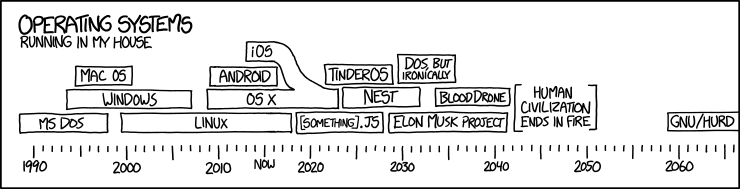
\includegraphics[scale=0.4]{imgs/xkcd_1508.png}
    \caption{\url{https://xkcd.com/1508/}}
  \end{figure}
\end{frame}

\begin{frame}[fragile]
  \frametitle{GNU HURD}

  HURD\@: Hird of Unix-Replacing Daemons

  HIRD\@: Hurd of Interfaces Representing Depth

  \begin{lstlisting}[mathescape=true,showstringspaces=false,numbers=none,frame=single]
  GNU HURD $:=$ [
    GNU  $:=$ GNU's Not Unix
    HURD $:=$ [
      HIRD $:=$ [
        HURD $:=$ [
          $\ldots$
        ] of Interfaces Representing Depth
      ] of Unix-Replacing Daemons
    ]
  ]
  \end{lstlisting}

\end{frame}

\begin{frame}
  \frametitle{Documentação}

  \begin{itemize}
    \item Horrível
    \item Escassa
    \item Conversas no IRC
    \item Confusa
    \item Alinear
    \item Feito pela comunidade
    \item Página de \textit{open issues}
    \item Recompensas (\$\$\$) para quem resolver
  \end{itemize}
\end{frame}

\section{Arquitetura Geral}

\begin{frame}
  \frametitle{Arquitetura do GNU Hurd}

  \begin{itemize}
    \item Microkernel (Mach)
    \item Multiservidor
    \item GNU C
    \item Servidores flexíveis (nível usuário)
    \item Servidores compilados como quiser
    \item MIG (Mach Interface Generator)
  \end{itemize}
\end{frame}

\section{Microkernel/Mach}

\begin{frame}
  \frametitle{Kernel}
  \begin{figure}[h]
    \hspace*{-0.9cm}
    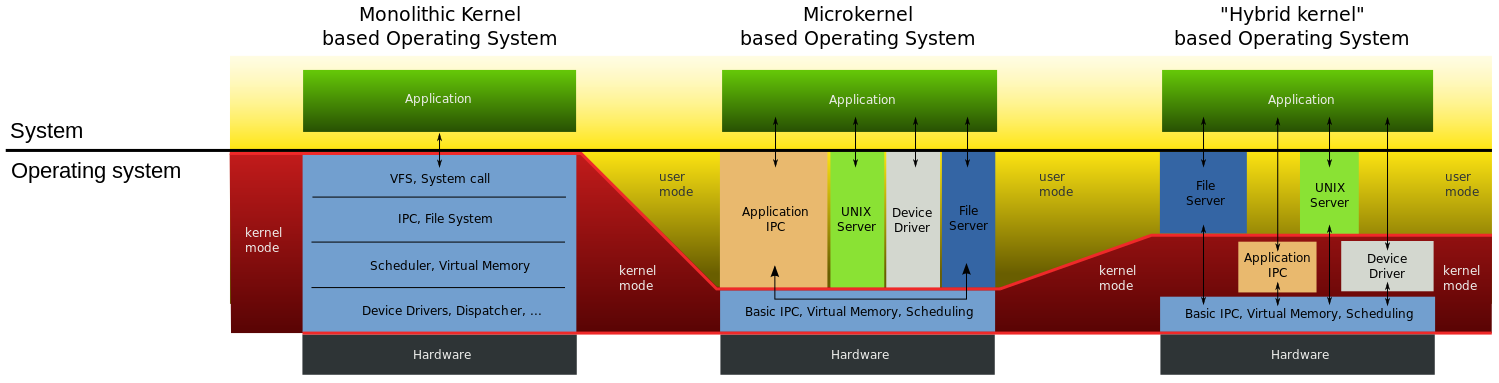
\includegraphics[scale=0.235]{imgs/kernel.png}
    \caption{\url{https://en.wikipedia.org/wiki/File:OS-structure2.svg}}
  \end{figure}
\end{frame}

\begin{frame}
  \frametitle{Comparação}
  \begin{description}
    \item[Microkernel] (e.g.\ Mach, kernel do Minix)
      \begin{itemize}
        \item Mais seguro
        \item Comunicação por mensagens (MIG)
        \item Responsabilidade bem definida
        \item Flexível (fácil de debugar os diferentes servidores)
        \item Mais estável
        \item Somente o absolutamente necessário
      \end{itemize}
    \item[Monolítico] (e.g.\ Linux)
      \begin{itemize}
        \item Não é necessário passar mensagem
        \item Mais rápido por ter acesso direto
        \item Código passa a se tornar complicado e confuso (spaghetti code)
        \item Pequenas (a às vezes aparentemente irrelevantes) mudanças podem quebrar o sistema
        \item Mais difícil de manter código
        \item Novos desenvolvedores sofrem tentando aprender código confuso
      \end{itemize}
  \end{description}
\end{frame}

\begin{frame}
  \frametitle{História do Mach}
  \begin{itemize}
    \item Criado em 1984 na Carnegie-Mellon
    \item Desenvolvimento do Mach terminou em 1994
    \item GNU Hurd usa GNU Mach (versão modificada para ser \textit{free} e manter-se atualizado)
    \item Microkernel/Nanokernel (alguns consideram ``Hybrid Kernel'')
    \item Mensagens por meio do MIG (Mach Interface Generator)
    \item MIG possibilita rodar código por RPC
  \end{itemize}
\end{frame}

\begin{frame}
  \frametitle{O que Mach faz e não faz?}
  \begin{description}
    \item[Faz:]~\\
      \begin{itemize}
        \item Gerenciamento de Memória
        \item Gerenciamento de Processos
        \item Comunicações (mensagens dos outros servidores)
        \item Entrada e Saída
      \end{itemize}
    \item [Não faz:]~\\
      \begin{itemize}
        \item Sistema de Arquivos
        \item Drivers
        \item Aplicativos de Usuário (WM, DE, etc.)
      \end{itemize}
  \end{description}
\end{frame}

\section{Multiservidor}

\begin{frame}
  \frametitle{Multiservidor}
  \begin{itemize}
    \item Rodam paralelamente ao Mach
    \item Comunicam-se pelo MIG
    \item Ficam na camada de usuário
    \item Qualquer linguagem
    \item Compilado como quiser
    \item Debugar enquanto os outros servidores rodam
    \item Independente de todos os outros servidores e kernel
    \item Completamente modificável
    \item Seguro (ficam em camada de usuário)
    \item Não é preciso dar reboot para testar
  \end{itemize}
\end{frame}

\begin{frame}
  \frametitle{Alguns exemplos de servidores}
  \begin{description}
    \item[Core]~\\
      \begin{itemize}
        \item \code{auth} privilégios, senhas e identificação
        \item \code{crash} erros
        \item \code{exec} rodar executáveis
        \item \code{fifo} pipes
        \item \code{firmlink} ``half-way between a symbolic link and hard link''
        \item \code{ifsock} sockets
        \item \code{init} boot
        \item \code{null} equivalente a \code{/dev/null} e \code{/dev/zero}
        \item \code{procs} PIDs
        \item \code{term} terminal
        \item $\ldots$
      \end{itemize}
    \item[Filesystem]~\\
      \begin{itemize}
        \item \code{ext2fs}, \code{isofs}, \code{nfs}, \code{ufs}, \code{ftpfs}, \code{storeio}
      \end{itemize}
  \end{description}
\end{frame}

\section{Memória}

\begin{frame}
  \frametitle{Memória no GNU Mach}
  \begin{itemize}
    \item 32-bit
    \item 2GB kernelspace
    \item 2GB userspace
    \item Mach cuida de toda memória virtual
    \item Pedidos de memória pelos processos feitos por mensagens
    \item Mach retorna um ponteiro para a memória e o tamanho alocado
  \end{itemize}
\end{frame}

\begin{frame}
  \frametitle{Escalonamento}
  Gerenciamento de memória por meio de uma Red-Black Tree (RBT) e usando Best-fit.

  Red-black tree é uma BST com espaço $\bigo(n)$ e operações $\bigo(\log n)$.

  Blocos: lista duplamente ligada.

  Usa-se uma RBT para ordenar os blocos em tamanho. Acha o melhor fit em tempo $\bigo(\log n)$.
  Modificar a lista é feito em $\bigo(1)$ já que é duplamente ligada.

  Complexidade final é $\bigo(\log n)$.

  (BSD, Linux, entre outros)
\end{frame}

\section{Escalonamento de Processos}

\begin{frame}
  \frametitle{Processos no GNU Mach}
  \begin{description}
    \item[Kernelspace:]~\\
      \begin{itemize}
        \item Usa \textit{continuations} (estrutura que guarda informação do processo)
        \item Continuations usam menos espaço pois não precisam da pilha de threads do kernel
        \item Não é preemptivo (por causa de continuations)
        \item Ser preemptivo requer toda a pilha de threads do kernel
        \item Escalonamento feito pelo Mach
        \item Escalonamento 1:1 (igual a Solaris, NetBSD, FreeBSD, OS X, iOS, OS/2 e Win32)
        \item Escalonamento feito por filas de prioridade
      \end{itemize}
  \end{description}
\end{frame}

\begin{frame}
  \frametitle{Processos no GNU Mach}
  \begin{description}
    \item[Userspace:]~\\
      \begin{itemize}
        \item Threads
        \item \code{libthreads}
        \item \code{libports}
        \item Servidores tem maior prioridade que user threads
        \item Não suporta múltiplas CPUs (anos 90)
      \end{itemize}
  \end{description}
\end{frame}

\section{Sistema de Arquivos}

\begin{frame}
  \frametitle{Filesystem no GNU Hurd}
  \begin{description}
    \item[Translators:]~\\
    \begin{itemize}
      \item Por \textit{i-nodes}
      \item Vários tradutores (servidores) para \code{fs}
      \item Cada tradutor é um tipo de formato
      \item Exemplos: \code{ext2fs}, \code{fatfs}, \code{ufs}, \code{isofs}
      \item Uma busca referencia uma \code{port} (uma porta para comunicar-se com o kernel)
    \end{itemize}
  \end{description}
\end{frame}

\begin{frame}
  \frametitle{Filesystem no GNU Hurd}
  A ideia: ao invés de uma lista telefônica contendo arquivos, temos uma árvore de busca que
  retorna uma porta para um servidor que pode acessar o arquivo.

  \begin{quote}
    ``So we don't have a single phone book listing all servers, but rather a tree of servers
    keeping track of each other. That's really like calling your friend and asking for the phone
    number of the blond girl at the party yesterday. He might refer you to a friend who hopefully
    knows more about it. Then you have to retry.''

    \hfill --- Markus Brinkmann
  \end{quote}
\end{frame}

\begin{frame}
  \frametitle{Filesystem no GNU Hurd}

  Usando-se uma árvore de busca de \textit{translators} possibilita algumas coisa bem
  interessantes:

  \begin{itemize}
    \item \code{nfs}
    \item \code{ftpfs}
  \end{itemize}

  Isso significa acesso transparente a servidores FTP no próprio filesystem. Usando-se o translator
  \code{ftpfs}, o usuário não precisa se preocupar com protocolos de rede.
\end{frame}

\section{Mensagens}

\begin{frame}
  \frametitle{O que o MIG (Mach Interface Generator) faz?}
  \begin{itemize}
    \item Serializa mensagens.
    \item Traduz mensagens.
    \item Envia mensagens.
    \item Recebe mensagens.
    \item Parecido com redes.
  \end{itemize}
\end{frame}

\begin{frame}[fragile]
  \frametitle{MIG (Mach Interface Generator)}
  \begin{lstlisting}[mathescape=true,showstringspaces=false,numbers=none,frame=single]
<teythoon> btw, I just realized that mig mashes two very different things
  together, namely the serialization/parsing and the message
  sending/receiving
<braunr> yes
<teythoon> I'd prefer it if that were separated
<braunr> me too
<braunr> that's why i want x15 to have a bare messaging interface .. :)
<teythoon> \o/
<braunr> simple (but optimized) scatter-gather
<braunr> it makes sense for mig since mach messages do include
  serialization metadata such as types
  \end{lstlisting}
\end{frame}

\begin{frame}
  \frametitle{MIG (Mach Interface Generator)}
  \begin{itemize}
    \item Processo 1 transforma código em mensagens.
    \item Mensagem é então enviada para processo 2.
    \item Mensagem é traduzida pelo MIG, gerando código C dentro do processo 2.
    \item Processo 2 roda o código.
  \end{itemize}
\end{frame}

\section{Comparação}

\begin{frame}
  \frametitle{GNU Hurd vs GNU/Linux}
  Vantagens do GNU Hurd em relação ao GNU/Linux:
  \begin{itemize}
    \item Microkernel
    \item Multiservidor
    \item Flexível
    \item Peças independentes entre si
    \item Comunidade entusiasmada
    \item Completamente GNU
  \end{itemize}
\end{frame}

\begin{frame}
  \frametitle{GNU Hurd vs GNU/Linux}
  Desvantagens do GNU Hurd em relação ao GNU/Linux:
  \begin{itemize}
    \item Menor performance
    \item Decisões antiquadas causaram problemas no futuro
    \item Minúscula comunidade e número de desenvolvedores
    \item Instável
    \item Falta muita coisa a ser feita
    \item Documentação escassa e ruim
  \end{itemize}
\end{frame}

%--------------------------------------------------------------------------------------------------

\section[Referências]{Referências e Bibliografia}
\begin{frame}[t,allowframebreaks]
  \frametitle{Referências e Bibliografia}
  \footnotesize
  \nocite{*}
  \printbibliography[]
\end{frame}

\end{document}
